\documentclass[]{article}
\usepackage{lmodern}
\usepackage{amssymb,amsmath}
\usepackage{ifxetex,ifluatex}
\usepackage{fixltx2e} % provides \textsubscript
\ifnum 0\ifxetex 1\fi\ifluatex 1\fi=0 % if pdftex
  \usepackage[T1]{fontenc}
  \usepackage[utf8]{inputenc}
\else % if luatex or xelatex
  \ifxetex
    \usepackage{mathspec}
  \else
    \usepackage{fontspec}
  \fi
  \defaultfontfeatures{Ligatures=TeX,Scale=MatchLowercase}
\fi
% use upquote if available, for straight quotes in verbatim environments
\IfFileExists{upquote.sty}{\usepackage{upquote}}{}
% use microtype if available
\IfFileExists{microtype.sty}{%
\usepackage{microtype}
\UseMicrotypeSet[protrusion]{basicmath} % disable protrusion for tt fonts
}{}
\usepackage[margin=1in]{geometry}
\usepackage{hyperref}
\hypersetup{unicode=true,
            pdftitle={Regression Final Project},
            pdfauthor={Joe DeMaro},
            pdfborder={0 0 0},
            breaklinks=true}
\urlstyle{same}  % don't use monospace font for urls
\usepackage{color}
\usepackage{fancyvrb}
\newcommand{\VerbBar}{|}
\newcommand{\VERB}{\Verb[commandchars=\\\{\}]}
\DefineVerbatimEnvironment{Highlighting}{Verbatim}{commandchars=\\\{\}}
% Add ',fontsize=\small' for more characters per line
\usepackage{framed}
\definecolor{shadecolor}{RGB}{248,248,248}
\newenvironment{Shaded}{\begin{snugshade}}{\end{snugshade}}
\newcommand{\KeywordTok}[1]{\textcolor[rgb]{0.13,0.29,0.53}{\textbf{#1}}}
\newcommand{\DataTypeTok}[1]{\textcolor[rgb]{0.13,0.29,0.53}{#1}}
\newcommand{\DecValTok}[1]{\textcolor[rgb]{0.00,0.00,0.81}{#1}}
\newcommand{\BaseNTok}[1]{\textcolor[rgb]{0.00,0.00,0.81}{#1}}
\newcommand{\FloatTok}[1]{\textcolor[rgb]{0.00,0.00,0.81}{#1}}
\newcommand{\ConstantTok}[1]{\textcolor[rgb]{0.00,0.00,0.00}{#1}}
\newcommand{\CharTok}[1]{\textcolor[rgb]{0.31,0.60,0.02}{#1}}
\newcommand{\SpecialCharTok}[1]{\textcolor[rgb]{0.00,0.00,0.00}{#1}}
\newcommand{\StringTok}[1]{\textcolor[rgb]{0.31,0.60,0.02}{#1}}
\newcommand{\VerbatimStringTok}[1]{\textcolor[rgb]{0.31,0.60,0.02}{#1}}
\newcommand{\SpecialStringTok}[1]{\textcolor[rgb]{0.31,0.60,0.02}{#1}}
\newcommand{\ImportTok}[1]{#1}
\newcommand{\CommentTok}[1]{\textcolor[rgb]{0.56,0.35,0.01}{\textit{#1}}}
\newcommand{\DocumentationTok}[1]{\textcolor[rgb]{0.56,0.35,0.01}{\textbf{\textit{#1}}}}
\newcommand{\AnnotationTok}[1]{\textcolor[rgb]{0.56,0.35,0.01}{\textbf{\textit{#1}}}}
\newcommand{\CommentVarTok}[1]{\textcolor[rgb]{0.56,0.35,0.01}{\textbf{\textit{#1}}}}
\newcommand{\OtherTok}[1]{\textcolor[rgb]{0.56,0.35,0.01}{#1}}
\newcommand{\FunctionTok}[1]{\textcolor[rgb]{0.00,0.00,0.00}{#1}}
\newcommand{\VariableTok}[1]{\textcolor[rgb]{0.00,0.00,0.00}{#1}}
\newcommand{\ControlFlowTok}[1]{\textcolor[rgb]{0.13,0.29,0.53}{\textbf{#1}}}
\newcommand{\OperatorTok}[1]{\textcolor[rgb]{0.81,0.36,0.00}{\textbf{#1}}}
\newcommand{\BuiltInTok}[1]{#1}
\newcommand{\ExtensionTok}[1]{#1}
\newcommand{\PreprocessorTok}[1]{\textcolor[rgb]{0.56,0.35,0.01}{\textit{#1}}}
\newcommand{\AttributeTok}[1]{\textcolor[rgb]{0.77,0.63,0.00}{#1}}
\newcommand{\RegionMarkerTok}[1]{#1}
\newcommand{\InformationTok}[1]{\textcolor[rgb]{0.56,0.35,0.01}{\textbf{\textit{#1}}}}
\newcommand{\WarningTok}[1]{\textcolor[rgb]{0.56,0.35,0.01}{\textbf{\textit{#1}}}}
\newcommand{\AlertTok}[1]{\textcolor[rgb]{0.94,0.16,0.16}{#1}}
\newcommand{\ErrorTok}[1]{\textcolor[rgb]{0.64,0.00,0.00}{\textbf{#1}}}
\newcommand{\NormalTok}[1]{#1}
\usepackage{graphicx,grffile}
\makeatletter
\def\maxwidth{\ifdim\Gin@nat@width>\linewidth\linewidth\else\Gin@nat@width\fi}
\def\maxheight{\ifdim\Gin@nat@height>\textheight\textheight\else\Gin@nat@height\fi}
\makeatother
% Scale images if necessary, so that they will not overflow the page
% margins by default, and it is still possible to overwrite the defaults
% using explicit options in \includegraphics[width, height, ...]{}
\setkeys{Gin}{width=\maxwidth,height=\maxheight,keepaspectratio}
\IfFileExists{parskip.sty}{%
\usepackage{parskip}
}{% else
\setlength{\parindent}{0pt}
\setlength{\parskip}{6pt plus 2pt minus 1pt}
}
\setlength{\emergencystretch}{3em}  % prevent overfull lines
\providecommand{\tightlist}{%
  \setlength{\itemsep}{0pt}\setlength{\parskip}{0pt}}
\setcounter{secnumdepth}{0}
% Redefines (sub)paragraphs to behave more like sections
\ifx\paragraph\undefined\else
\let\oldparagraph\paragraph
\renewcommand{\paragraph}[1]{\oldparagraph{#1}\mbox{}}
\fi
\ifx\subparagraph\undefined\else
\let\oldsubparagraph\subparagraph
\renewcommand{\subparagraph}[1]{\oldsubparagraph{#1}\mbox{}}
\fi

%%% Use protect on footnotes to avoid problems with footnotes in titles
\let\rmarkdownfootnote\footnote%
\def\footnote{\protect\rmarkdownfootnote}

%%% Change title format to be more compact
\usepackage{titling}

% Create subtitle command for use in maketitle
\newcommand{\subtitle}[1]{
  \posttitle{
    \begin{center}\large#1\end{center}
    }
}

\setlength{\droptitle}{-2em}

  \title{Regression Final Project}
    \pretitle{\vspace{\droptitle}\centering\huge}
  \posttitle{\par}
    \author{Joe DeMaro}
    \preauthor{\centering\large\emph}
  \postauthor{\par}
      \predate{\centering\large\emph}
  \postdate{\par}
    \date{April 4, 2019}


\begin{document}
\maketitle

\subsection{Executive Summary}\label{executive-summary}

You work for Motor Trend, a magazine about the automobile industry.
Looking at a data set of a collection of cars, they are interested in
exploring the relationship between a set of variables and miles per
gallon (MPG) (outcome). They are particularly interested in the
following two questions:

``Is an automatic or manual transmission better for MPG''

``Quantify the MPG difference between automatic and manual
transmissions''

To investigate the first question, a comparison of the raw data is used
to drive a linear regression comparsion between the two variables within
the inquire. The inital analysis shows a 7.25 mpg difference between
manual and automatic transmissson. The p-value for the comparison is
0.0014 indicating the difference is significant. The regression data
indicates this comparison only account for \textasciitilde{}35\% of the
differences. The initial pass does not help determine if any other
measurement affects mpg. To determine if other factors might affect MPG,
a regression model is executed with all variables considered. The
information from this model (mod1) led to significant differences being
seen between mpg and wgt, cyl, and disp. These 3 variables were modeled
with am to identify other variables affecting mpg. wgt and cyl
significantly affect mpg and the data show the 4 variables account for
over 80\% of the differences in mpg Residual analysis plot show that the
data are non problematic and linear regression modeling is appropriate.

\section{Appendix}\label{appendix}

\subsection{Exploratory Data
Visualization}\label{exploratory-data-visualization}

\begin{Shaded}
\begin{Highlighting}[]
\KeywordTok{head}\NormalTok{(mtcars)}
\end{Highlighting}
\end{Shaded}

\begin{verbatim}
##                    mpg cyl disp  hp drat    wt  qsec vs am gear carb
## Mazda RX4         21.0   6  160 110 3.90 2.620 16.46  0  1    4    4
## Mazda RX4 Wag     21.0   6  160 110 3.90 2.875 17.02  0  1    4    4
## Datsun 710        22.8   4  108  93 3.85 2.320 18.61  1  1    4    1
## Hornet 4 Drive    21.4   6  258 110 3.08 3.215 19.44  1  0    3    1
## Hornet Sportabout 18.7   8  360 175 3.15 3.440 17.02  0  0    3    2
## Valiant           18.1   6  225 105 2.76 3.460 20.22  1  0    3    1
\end{verbatim}

\begin{Shaded}
\begin{Highlighting}[]
\KeywordTok{str}\NormalTok{(mtcars)}
\end{Highlighting}
\end{Shaded}

\begin{verbatim}
## 'data.frame':    32 obs. of  11 variables:
##  $ mpg : num  21 21 22.8 21.4 18.7 18.1 14.3 24.4 22.8 19.2 ...
##  $ cyl : num  6 6 4 6 8 6 8 4 4 6 ...
##  $ disp: num  160 160 108 258 360 ...
##  $ hp  : num  110 110 93 110 175 105 245 62 95 123 ...
##  $ drat: num  3.9 3.9 3.85 3.08 3.15 2.76 3.21 3.69 3.92 3.92 ...
##  $ wt  : num  2.62 2.88 2.32 3.21 3.44 ...
##  $ qsec: num  16.5 17 18.6 19.4 17 ...
##  $ vs  : num  0 0 1 1 0 1 0 1 1 1 ...
##  $ am  : num  1 1 1 0 0 0 0 0 0 0 ...
##  $ gear: num  4 4 4 3 3 3 3 4 4 4 ...
##  $ carb: num  4 4 1 1 2 1 4 2 2 4 ...
\end{verbatim}

\begin{Shaded}
\begin{Highlighting}[]
\NormalTok{data.subset <-}\StringTok{ }\KeywordTok{subset}\NormalTok{(mtcars, }\DataTypeTok{select=}\KeywordTok{c}\NormalTok{(mpg,am))}
\NormalTok{mt.auto <-}\StringTok{ }\NormalTok{mtcars[(mtcars}\OperatorTok{$}\NormalTok{am}\OperatorTok{==}\DecValTok{0}\NormalTok{),]}
\NormalTok{mt.manual <-}\StringTok{ }\NormalTok{mtcars[(mtcars}\OperatorTok{$}\NormalTok{am}\OperatorTok{==}\DecValTok{1}\NormalTok{),]}

\KeywordTok{boxplot}\NormalTok{(mpg }\OperatorTok{~}\StringTok{ }\NormalTok{am, }\DataTypeTok{data=}\NormalTok{mtcars, }\DataTypeTok{xlab=}\StringTok{"Transmission"}\NormalTok{, }\DataTypeTok{ylab=}\StringTok{"MPG"}\NormalTok{, }\DataTypeTok{main=}\StringTok{"MPG v Transmission Type"}\NormalTok{)}
\end{Highlighting}
\end{Shaded}

\includegraphics{regressionFinal_files/figure-latex/mtcars-1.pdf}

\begin{Shaded}
\begin{Highlighting}[]
\KeywordTok{summary}\NormalTok{(mtcars)}
\end{Highlighting}
\end{Shaded}

\begin{verbatim}
##       mpg             cyl             disp             hp       
##  Min.   :10.40   Min.   :4.000   Min.   : 71.1   Min.   : 52.0  
##  1st Qu.:15.43   1st Qu.:4.000   1st Qu.:120.8   1st Qu.: 96.5  
##  Median :19.20   Median :6.000   Median :196.3   Median :123.0  
##  Mean   :20.09   Mean   :6.188   Mean   :230.7   Mean   :146.7  
##  3rd Qu.:22.80   3rd Qu.:8.000   3rd Qu.:326.0   3rd Qu.:180.0  
##  Max.   :33.90   Max.   :8.000   Max.   :472.0   Max.   :335.0  
##       drat             wt             qsec             vs        
##  Min.   :2.760   Min.   :1.513   Min.   :14.50   Min.   :0.0000  
##  1st Qu.:3.080   1st Qu.:2.581   1st Qu.:16.89   1st Qu.:0.0000  
##  Median :3.695   Median :3.325   Median :17.71   Median :0.0000  
##  Mean   :3.597   Mean   :3.217   Mean   :17.85   Mean   :0.4375  
##  3rd Qu.:3.920   3rd Qu.:3.610   3rd Qu.:18.90   3rd Qu.:1.0000  
##  Max.   :4.930   Max.   :5.424   Max.   :22.90   Max.   :1.0000  
##        am              gear            carb      
##  Min.   :0.0000   Min.   :3.000   Min.   :1.000  
##  1st Qu.:0.0000   1st Qu.:3.000   1st Qu.:2.000  
##  Median :0.0000   Median :4.000   Median :2.000  
##  Mean   :0.4062   Mean   :3.688   Mean   :2.812  
##  3rd Qu.:1.0000   3rd Qu.:4.000   3rd Qu.:4.000  
##  Max.   :1.0000   Max.   :5.000   Max.   :8.000
\end{verbatim}

\subsection{Compare Auto vs.~Manual
Transmission}\label{compare-auto-vs.manual-transmission}

\begin{Shaded}
\begin{Highlighting}[]
\KeywordTok{aggregate}\NormalTok{(data.subset[,}\DecValTok{1}\OperatorTok{:}\DecValTok{2}\NormalTok{], }\KeywordTok{list}\NormalTok{(data.subset}\OperatorTok{$}\NormalTok{am), mean)}
\end{Highlighting}
\end{Shaded}

\begin{verbatim}
##   Group.1      mpg am
## 1       0 17.14737  0
## 2       1 24.39231  1
\end{verbatim}

\begin{Shaded}
\begin{Highlighting}[]
\NormalTok{mod0 <-}\StringTok{ }\KeywordTok{lm}\NormalTok{(mpg }\OperatorTok{~}\StringTok{ }\NormalTok{am, mtcars)}
\KeywordTok{summary}\NormalTok{(mod0)}
\end{Highlighting}
\end{Shaded}

\begin{verbatim}
## 
## Call:
## lm(formula = mpg ~ am, data = mtcars)
## 
## Residuals:
##     Min      1Q  Median      3Q     Max 
## -9.3923 -3.0923 -0.2974  3.2439  9.5077 
## 
## Coefficients:
##             Estimate Std. Error t value Pr(>|t|)    
## (Intercept)   17.147      1.125  15.247 1.13e-15 ***
## am             7.245      1.764   4.106 0.000285 ***
## ---
## Signif. codes:  0 '***' 0.001 '**' 0.01 '*' 0.05 '.' 0.1 ' ' 1
## 
## Residual standard error: 4.902 on 30 degrees of freedom
## Multiple R-squared:  0.3598, Adjusted R-squared:  0.3385 
## F-statistic: 16.86 on 1 and 30 DF,  p-value: 0.000285
\end{verbatim}

\begin{Shaded}
\begin{Highlighting}[]
\KeywordTok{t.test}\NormalTok{(mt.auto}\OperatorTok{$}\NormalTok{mpg, mt.manual}\OperatorTok{$}\NormalTok{mpg)}
\end{Highlighting}
\end{Shaded}

\begin{verbatim}
## 
##  Welch Two Sample t-test
## 
## data:  mt.auto$mpg and mt.manual$mpg
## t = -3.7671, df = 18.332, p-value = 0.001374
## alternative hypothesis: true difference in means is not equal to 0
## 95 percent confidence interval:
##  -11.280194  -3.209684
## sample estimates:
## mean of x mean of y 
##  17.14737  24.39231
\end{verbatim}

\begin{Shaded}
\begin{Highlighting}[]
\NormalTok{diffTrans <-}\StringTok{ }\KeywordTok{mean}\NormalTok{(mt.manual}\OperatorTok{$}\NormalTok{mpg) }\OperatorTok{-}\StringTok{ }\KeywordTok{mean}\NormalTok{(mt.auto}\OperatorTok{$}\NormalTok{mpg)}
\NormalTok{### Difference between manual and automatic transmission}
\NormalTok{diffTrans}
\end{Highlighting}
\end{Shaded}

\begin{verbatim}
## [1] 7.244939
\end{verbatim}

\subsection{Effect of Multiple
Variables}\label{effect-of-multiple-variables}

\subsubsection{Initial comparison driven by the questions of interest
provide limited insight into the mtcars data. With additional data
available and the linear regression results of mod0 indicating only 35\%
of the difference in mpg can be explained by am, a more complete
analysis will be gleaned by looking at a broad comparison of all the
variables and then determining a more filtered view based on the
additional
information.}\label{initial-comparison-driven-by-the-questions-of-interest-provide-limited-insight-into-the-mtcars-data.-with-additional-data-available-and-the-linear-regression-results-of-mod0-indicating-only-35-of-the-difference-in-mpg-can-be-explained-by-am-a-more-complete-analysis-will-be-gleaned-by-looking-at-a-broad-comparison-of-all-the-variables-and-then-determining-a-more-filtered-view-based-on-the-additional-information.}

\begin{Shaded}
\begin{Highlighting}[]
\NormalTok{mod1 <-}\StringTok{ }\KeywordTok{lm}\NormalTok{(mpg}\OperatorTok{~}\NormalTok{cyl }\OperatorTok{+}\StringTok{ }\NormalTok{disp }\OperatorTok{+}\StringTok{ }\NormalTok{hp }\OperatorTok{+}\StringTok{ }\NormalTok{drat }\OperatorTok{+}\StringTok{ }\NormalTok{wt }\OperatorTok{+}\StringTok{ }\NormalTok{qsec }\OperatorTok{+}\StringTok{ }\NormalTok{vs }\OperatorTok{+}\StringTok{ }\NormalTok{am }\OperatorTok{+}\StringTok{ }\NormalTok{gear }\OperatorTok{+}\StringTok{ }\NormalTok{carb, }\DataTypeTok{data=}\NormalTok{mtcars)}
\KeywordTok{summary}\NormalTok{(mod1)}\OperatorTok{$}\NormalTok{coef}
\end{Highlighting}
\end{Shaded}

\begin{verbatim}
##                Estimate  Std. Error    t value   Pr(>|t|)
## (Intercept) 12.30337416 18.71788443  0.6573058 0.51812440
## cyl         -0.11144048  1.04502336 -0.1066392 0.91608738
## disp         0.01333524  0.01785750  0.7467585 0.46348865
## hp          -0.02148212  0.02176858 -0.9868407 0.33495531
## drat         0.78711097  1.63537307  0.4813036 0.63527790
## wt          -3.71530393  1.89441430 -1.9611887 0.06325215
## qsec         0.82104075  0.73084480  1.1234133 0.27394127
## vs           0.31776281  2.10450861  0.1509915 0.88142347
## am           2.52022689  2.05665055  1.2254035 0.23398971
## gear         0.65541302  1.49325996  0.4389142 0.66520643
## carb        -0.19941925  0.82875250 -0.2406258 0.81217871
\end{verbatim}

\begin{Shaded}
\begin{Highlighting}[]
\KeywordTok{summary}\NormalTok{(}\KeywordTok{aov}\NormalTok{(mod1))}
\end{Highlighting}
\end{Shaded}

\begin{verbatim}
##             Df Sum Sq Mean Sq F value   Pr(>F)    
## cyl          1  817.7   817.7 116.425 5.03e-10 ***
## disp         1   37.6    37.6   5.353  0.03091 *  
## hp           1    9.4     9.4   1.334  0.26103    
## drat         1   16.5    16.5   2.345  0.14064    
## wt           1   77.5    77.5  11.031  0.00324 ** 
## qsec         1    3.9     3.9   0.562  0.46166    
## vs           1    0.1     0.1   0.018  0.89317    
## am           1   14.5    14.5   2.061  0.16586    
## gear         1    1.0     1.0   0.138  0.71365    
## carb         1    0.4     0.4   0.058  0.81218    
## Residuals   21  147.5     7.0                     
## ---
## Signif. codes:  0 '***' 0.001 '**' 0.01 '*' 0.05 '.' 0.1 ' ' 1
\end{verbatim}

\subsection{Deeper Analysis}\label{deeper-analysis}

\subsubsection{The analysis of variance from the regression model (mod1)
shows 3 significantly different factors. A new model (mod2) below will
limit x variables to the 3 discovered variables plus am, part of the
original question. The results show that transmission type plus number
of cylinders and weight have a significant impact on
MPG}\label{the-analysis-of-variance-from-the-regression-model-mod1-shows-3-significantly-different-factors.-a-new-model-mod2-below-will-limit-x-variables-to-the-3-discovered-variables-plus-am-part-of-the-original-question.-the-results-show-that-transmission-type-plus-number-of-cylinders-and-weight-have-a-significant-impact-on-mpg}

\begin{Shaded}
\begin{Highlighting}[]
\NormalTok{mod2 <-}\StringTok{ }\KeywordTok{lm}\NormalTok{(mpg }\OperatorTok{~}\StringTok{ }\KeywordTok{factor}\NormalTok{(am) }\OperatorTok{+}\StringTok{ }\NormalTok{cyl }\OperatorTok{+}\StringTok{ }\NormalTok{disp }\OperatorTok{+}\StringTok{ }\NormalTok{wt, mtcars)}
\KeywordTok{summary}\NormalTok{(mod2)}
\end{Highlighting}
\end{Shaded}

\begin{verbatim}
## 
## Call:
## lm(formula = mpg ~ factor(am) + cyl + disp + wt, data = mtcars)
## 
## Residuals:
##    Min     1Q Median     3Q    Max 
## -4.318 -1.362 -0.479  1.354  6.059 
## 
## Coefficients:
##              Estimate Std. Error t value Pr(>|t|)    
## (Intercept) 40.898313   3.601540  11.356 8.68e-12 ***
## factor(am)1  0.129066   1.321512   0.098  0.92292    
## cyl         -1.784173   0.618192  -2.886  0.00758 ** 
## disp         0.007404   0.012081   0.613  0.54509    
## wt          -3.583425   1.186504  -3.020  0.00547 ** 
## ---
## Signif. codes:  0 '***' 0.001 '**' 0.01 '*' 0.05 '.' 0.1 ' ' 1
## 
## Residual standard error: 2.642 on 27 degrees of freedom
## Multiple R-squared:  0.8327, Adjusted R-squared:  0.8079 
## F-statistic: 33.59 on 4 and 27 DF,  p-value: 4.038e-10
\end{verbatim}

\begin{Shaded}
\begin{Highlighting}[]
\KeywordTok{summary}\NormalTok{(}\KeywordTok{aov}\NormalTok{(mod2))}
\end{Highlighting}
\end{Shaded}

\begin{verbatim}
##             Df Sum Sq Mean Sq F value   Pr(>F)    
## factor(am)   1  405.2   405.2  58.055 3.40e-08 ***
## cyl          1  449.5   449.5  64.415 1.26e-08 ***
## disp         1   19.3    19.3   2.763  0.10805    
## wt           1   63.7    63.7   9.121  0.00547 ** 
## Residuals   27  188.4     7.0                     
## ---
## Signif. codes:  0 '***' 0.001 '**' 0.01 '*' 0.05 '.' 0.1 ' ' 1
\end{verbatim}

\begin{Shaded}
\begin{Highlighting}[]
\KeywordTok{anova}\NormalTok{(mod0,mod2)}
\end{Highlighting}
\end{Shaded}

\begin{verbatim}
## Analysis of Variance Table
## 
## Model 1: mpg ~ am
## Model 2: mpg ~ factor(am) + cyl + disp + wt
##   Res.Df    RSS Df Sum of Sq      F    Pr(>F)    
## 1     30 720.90                                  
## 2     27 188.43  3    532.47 25.433 5.034e-08 ***
## ---
## Signif. codes:  0 '***' 0.001 '**' 0.01 '*' 0.05 '.' 0.1 ' ' 1
\end{verbatim}

\subsection{Residual Analysis}\label{residual-analysis}

\begin{Shaded}
\begin{Highlighting}[]
\KeywordTok{par}\NormalTok{(}\DataTypeTok{mfrow=}\KeywordTok{c}\NormalTok{(}\DecValTok{2}\NormalTok{,}\DecValTok{2}\NormalTok{))}
\KeywordTok{plot}\NormalTok{(mod2)}
\end{Highlighting}
\end{Shaded}

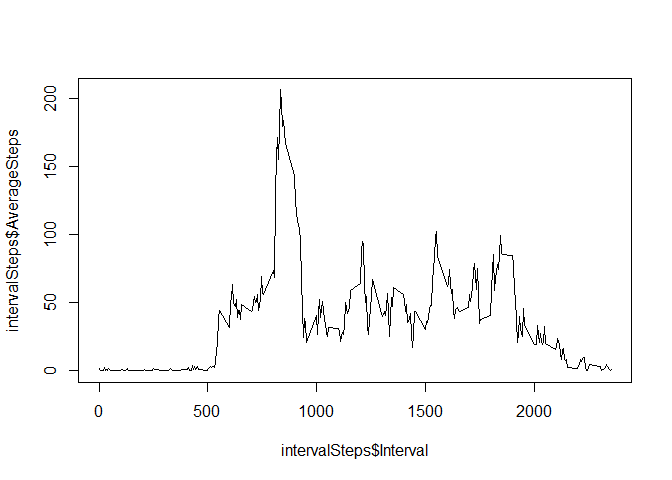
\includegraphics{regressionFinal_files/figure-latex/unnamed-chunk-4-1.pdf}


\end{document}
